
\documentclass[12pt,a4paper,twoside]{article}

%\usepackage[polish]{babel}
\usepackage[utf8x]{inputenc}
\usepackage[T1]{fontenc}
\usepackage{fdsymbol}       % Contains a symbol for ⌀ -- use \diameter
\usepackage{newunicodechar} % To write the definition on the next line
\usepackage{graphicx} 
\title{Boże Królestwo na Polskiej Ziemi: Wpływ Chrześcijaństwa na Dzieje Polski}
\author{Michał Kraus}
\date{2024.12.19}

\usepackage[a4paper,
            inner=3cm,
            outer=1cm,
            top=1cm,
            bottom=1.6cm]{geometry}

\usepackage{multicol}
\linespread{1}
\usepackage{enumitem}

\begin{document}

\maketitle

\begin{center}
    wstęp
\end{center}

Celem niniejszej pracy jest przedstawienie wpływu Kościoła rzymskokatolickiego na rozwój i kształtowanie się polskiej tożsamości narodowej oraz kulturowej. Analizując ten wpływ, skupię się na znaczeniu religii katolickiej w kontekście historycznym, cywilizacyjnym i społecznym. Zawarte w pracy rozważania obejmą m.in. rolę Kościoła w tworzeniu fundamentów państwowości polskiej, jego wpływ na kulturę, edukację oraz na kształtowanie wartości narodowych.
W pracy uwzględnię argumenty oparte na szerokim zakresie źródeł – od tekstów teologicznych po prace historyków i socjologów, których badania pozwalają na pełniejsze zrozumienie roli Kościoła w polskim życiu społecznym. W kontekście współczesnym, omówię również wyzwania, przed którymi stoi Kościół katolicki w Polsce, oraz zmieniające się relacje między religią a społeczeństwem.
Pisząc tę pracę, mam nadzieję zachęcić czytelników do refleksji nad rolą Kościoła w kształtowaniu polskiej tożsamości oraz do zastanowienia się nad miejscem religii w dzisiejszym społeczeństwie.



\tableofcontents


%\begin{multicols}{2}


\section{Rozdział Chrzest jako narodziny Polski}

\subsection{Wprowadzenie: Narodziny Polski i symboliczna data chrztu}

\begin{figure}

    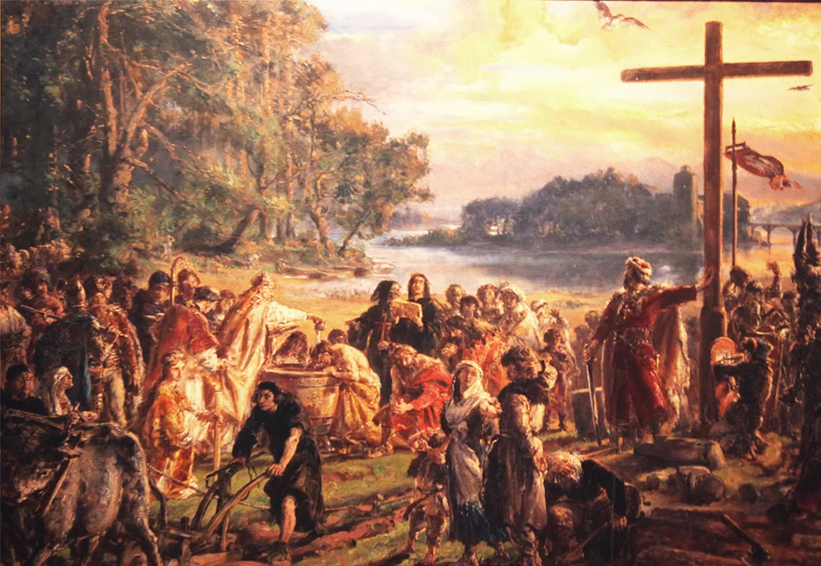
\includegraphics[width=8cm, height=8cm]{Polska_poczatek.png}
\end{figure}

„Każdy Polak powinien być świadomy, jak Polska się narodziła, kiedy i w jakich okolicznościach. Symboliczną datą powstania Polski jako państwa chrześcijańskiego jest rok 966, kiedy Mieszko I przyjął chrzest. Jak zauważa dr hab. Grzegorz Pac, średniowieczne źródła dotyczące tego wydarzenia są skromne i historycy niejednokrotnie muszą opierać się na domysłach i przypuszczeniach.

Niemniej jednak, pewnym faktem jest przyjęcie chrztu przez Mieszka I, które miało fundamentalne znaczenie dla kształtowania tożsamości i charakteru narodu polskiego. Chrzest Polski oznaczał nie tylko włączenie młodego państwa do wspólnoty chrześcijańskich narodów Europy, ale także zapoczątkowanie przemian w strukturze społecznej i prawnej, opartych na wartościach chrześcijańskich.”

\subsection{Przyczyny chrztu i jego znaczenie polityczne}

Decyzja Mieszka I o przyjęciu chrztu miała nie tylko charakter religijny, ale również polityczny. Przyjęcie chrześcijaństwa umożliwiło Polsce zbliżenie się do chrześcijańskiej Europy i zawiązanie sojuszy, co miało kluczowe znaczenie dla stabilizacji i bezpieczeństwa nowo powstałego państwa. Mieszko mógł w ten sposób poślubić księżniczkę Dobrawę, córkę księcia czeskiego, co umocniło pozycję Polski na arenie międzynarodowej i zapewniło jej ochronę przed atakami ze strony pogan. Jednakże jak zauważył dr. hab. Pac konwersja tamtego społeczeństwa z pogańskiego na chrześcijański wymagał silnego władcy, który był w stanie narzucić nowe prawo oparte o wartości i etykę chrześcijańską. W przeciwnym razie doszłoby do podziału społeczeństwa na dwie grupy, które by żyły według dwóch różnych porządków. co prowadziłoby do chaosu i konfliktów wewnętrznych. Lud musiał pójść w ślady za swym władcą, aby mógł zapanować porządek i jedność. Chrystianizacja Polski przebiegała powoli, ale zdecydowanie.

\subsection{Chrystianizacja Polski i jej wpływ na tożsamość narodową}

Chrzest Mieszka I, zwany również „Chrztem Polski”, nadał nowopowstałemu państwu charakter wyznaniowy. Wydarzenie to odcisnęło ponadczasowe piętno na Polsce i jej narodzie, łącząc go nierozerwalnie z chrześcijaństwem i jego dziedzictwem. W kolejnych stuleciach chrześcijaństwo kształtowało etykę, kulturę, światopogląd oraz tradycję Polek i Polaków. Jak ujął to papież Jan Paweł II:
„Chrzest Polski, który dokonał się w 966 roku, jest faktem o fundamentalnym znaczeniu w historii naszego narodu, w jego kulturze, w jego tożsamości, w jego przynależności do chrześcijaństwa. Mieszko I, w tym wielkim akcie, nie tylko wprowadził Polskę do rodziny narodów chrześcijańskich, ale równocześnie nadał narodowi polskiemu charakter, który przez wieki, przez wieki będzie w sposób nieodwracalny stanowił o jego tożsamości.”



\subsection{Rozwój chrześcijaństwa w Polsce: „Bóg, Honor, Ojczyzna”}

Od czasu chrztu Polska rozwijała się jako kraj chrześcijański. Powstawały kościoły, na budynkach stawiano krzyże, a wiara stawała się nieodłącznym elementem polskiej kultury i tradycji. Słowa „Bóg, Honor, Ojczyzna” stały się hasłem, które wyrażało system wartości Polaków i odróżniało naród polski od innych narodów. Należy podkreślić, że „Bóg” umieszczany jest na pierwszym miejscu, symbolizując jego centralną rolę w życiu duchowym i moralnym Polaków.

\section{Rozdział 2 Dziedzictwo kulturowe i artystyczne Kościoła w Polsce.}

W tym rozdziale skoncentruję się na materialnym i artystycznym dziedzictwie, jakie Kościół pozostawił w Polsce. Architektura, malarstwo oraz literatura inspirowane chrześcijańskimi wartościami stanowią wyjątkowe świadectwo wpływu wiary na polską kulturę. Poprzez prezentację wybranych przykładów tych dziedzin postaram się ukazać piękno i głębię twórczości, która czerpała z religijnej duchowości i tradycji.

\subsection{Sakralna architektura: Katedry i kościoły jako perły polskiego dziedzictwa}

Jak wspominałem wiara dotyczyła niemal każdego aspektu społecznego także tego jak postrzegano piękno, symbolikę. Pewnego rodzaju konsekwencją Chrystianizacji Europy w tym i Polski było powstanie Gotyku . Gotyk, który był rozpowszechniany między innymi przez zakonników benedyktynów i cystersów.
W stylu gotyckim budowano nie tylko kościoły i piękne katedry, ale także zamki, jak Zamek Kapituły Warmińskiej czy Zamek krzyżacki w Kętrzynie. Można wymienić wiele innych przykładów. Piękno tego stylu chciałbym ukazać na przykładzie dwóch obiektów w Polsce.
Pierwszym takim pierwszym miejscem będzie Katedra jaką zamierzam wziąć pod lupę jest katedra Wawelska (Kraków). Jej budowa rozpoczęła się w XI wieku, a obecna gotycka forma pochodzi głównie z XIV wieku. Obecna forma Katedry Wawelskiej (gotycka) to wynik przebudowy rozpoczętej w XIV wieku, ale w kontekście chrześcijaństwa była ona również rozwijana przez inne style, np. romański i renesansowy. Jest to miejsce koronacji Polskich królów, ale także i miejsce, gdzie pochowano wiele ważnych osobistości.  Katedra jest trójnawową gotycką bazyliką, wykonaną z cegły i kamienia wapiennego.  Charakterystyczne gotyckie łuki wsparte na cienkich filarach symbolizują dążenie ku niebu. Przestrzeń w niej wydaje się bardzo duża, a jej wnętrze jest bogato ozdobione. Ponadto posiada ona wielkie witraże które pozwalają na dopływ dużej ilości światła, które ma symbolizować boską obecność.  Jak zaznaczył prof. Michał Rożek w swojej książce „Krakowska Katedra na Wawelu” Katedra ma bogatą symbolikę tego miejsca jako centrum polskiej historii, kultury i duchowości.

Jako drugiemu przyjrzymy się Kościołowi Mariackiemu (Kraków).  Kościół Mariacki w Krakowie jest jednym z najważniejszych i najpiękniejszych zabytków w Polsce, z bogatą historią sięgającą średniowiecza. Pierwsze wzmianki o kościele pochodzą z 1222 roku, kiedy był jeszcze romańską świątynią. Obiekt ten został zniszczony podczas najazdów tatarskich, a jego odbudowę rozpoczęto w XIII wieku. Obecna gotycka forma pochodzi głównie z XIV wieku, kiedy budowę wspierali krakowscy mieszczanie, m.in. poprzez bogate fundacje i mecenat artystyczny. W XV wieku dodano ośmioboczną kondygnację wieży hejnałowej oraz charakterystyczny gotycki hełm. Kościół słynie z unikalnego ołtarza głównego autorstwa Wita Stwosza, który został wykonany w latach 1477–1489. Jest to najwybitniejsze dzieło późnogotyckiej rzeźby w Europie 
Środkowej, przedstawiające sceny z życia Marii i Chrystusa.

	Pięknych kościołów oraz innych obiektów gotyckich jest w Polsce bardzo wiele, a ich liczba świadczy o głębokim wpływie chrześcijaństwa na sztukę i kulturę średniowieczną. Można godzinami analizować ich majestatyczne konstrukcje oraz duchowe przesłanie, jakie niosą. Jednak zakończę omawianie architektury, aby skupić się na innych aspektach, w których Kościół katolicki wpłynął na kształtowanie historii, kultury i tożsamości narodowej Polski.
\subsection{Literatura polska inspirowana wiarą i duchowością}

Warto wspomnieć, iż w czasach średniowiecza większość jak i być może cała literatura krajów europejskich była pisana w języku Łacińskim do dziś uważanego za język Świętego Kościoła. Także i wiele Polskich średniowiecznych twórców literackich pisało utwory tylko w języku łacińskim który był w tamtej epoce uniwersalny. Dopiero w Polsce zdaje się złamał Jan Kochanowski, którego uważa się za twórcę języka polskiego literackiego. Autor w swoich dziełach odwoływał się wielokrotnie do filozofii stoickiej i chrześcijańskiej. 
Sądzę, że niemal każdy Polak słyszał o takich twórcach jak Jan Kochanowski, Adam Mickiewicz, Wacław Potocki oraz wiele innych wybitnych Polskich twórców. W ich dziełach często możemy znaleźć odniesienia do Biblii, tradycji katolickiej i symboliki. Przykładowo w utworze Dziady cz. III Adama Mickiewicza, znajdziemy liczne nawiązania do Mesjanizmu (w ów utworze możemy znaleźć motyw Polski Chrystusem narodów. Porównanie Polski do ukrzyżowanego Jezusa. Bardzo znamienna jest scena wizji księdza Piotra. Ta scena ukazuje Polskę jako duchowego odkupiciela narodów), elementy takie jak Anioły, Demony oraz wiele innych.

\begin{itemize}
    \item Anonimowy autor „Bogurodzicy” – najstarsza polska pieśń religijna (XIII–XIV w.), uznawana za symbol wiary narodowej i modlitwy do Matki Bożej. Przez pewien okres ów utwór pełnił bardzo ważną funkcję w Polsce jako hymnu narodowego.
    \item Jan Kochanowski – w „Trenach” opłakiwał swoją zmarłą córkę Urszulę, poruszając kwestie wiary, nieśmiertelności duszy i zaufania do Bożej opatrzności. Jego „Pieśni” zawierają liczne nawiązania religijne.
    \item Jan Andrzej Morsztyn – poeta, który w swoich wierszach religijnych, takich jak „Pieśni pokutne,” ukazywał swoje zmagania duchowe i skruchę.
    \item Henryk Sienkiewicz – w powieści „Quo Vadis” odwołuje się do początków chrześcijaństwa, ukazując konfrontację wiary chrześcijańskiej z pogańskim Rzymem.


  \end{itemize}
  
\section{Historia Izraela a Polska: Wiara i losy narodów}






%\end{multicols}


\end{document}



